\chapter{Board Representation}
A chess program requires an internal board representation to maintain the current locations of each piece and also additional information to identify whose turn it is to play, castling rights and whether an en passant move is possible. Furthermore, more advanced engines require additional data structures to keep track of previous moves in order to avoid \textit{threefold repetition} and the \textit{fifty-move rule}.
\section{Array}
The most intuitive board representation would be a $8 \times 8$ 2-dimensional array of 1 byte words. This board representation was the first design that had come to my mind. This design would also be quite space efficient, which was a big consideration for me as the \textit{Monte Carlo Tree Search} algorithm requires a tree data structure to be kept, with each \textit{node} containing a full board representation.\\\\
This particular board representation would allow for the whole board to be represented by \textbf{64 bytes} in total, as there are 64 slots of 1 byte each. As there are only 12 different types of pieces, only 4 bits are required to determine the colour of the piece and the type of the piece. This allows for the board to be represented with a lower byte count of \textbf{32 bytes} if we were to use 4 bit words for each cell of the array. Whereas this would be faster for systems that are optimised for 4 bit words, most modern systems and hardware is designed to handle 8-64 bit words, and therefore I would have chosen to take the larger sized array for higher speed if I had decided to use this design. Furthermore, more bits would be required to hold the additional information about the state of the game.\\\\
Despite the small size of the board representation, speed, which is arguably a greater concern when designing chess engines is much slower as opposed to using bitboards. This is because when we generate possible moves, it is necessary to loop through each cell, identify whether a piece exists within the cell, and if a piece does exist, then generate the possible destinations and create copies of the board for each destination that can be made for the selected piece. This must be done for each and every piece and unlike bitboards, we cannot use simple bitwise operations which are usually single instructions and requires much less overhead.

\section{Bitboards}
Bitboards are an array of 64-bit words that can represent the chess board. Because there are 2 colours and 6 different types of pieces, the usual bitboard representation consists of an array of 12 64-bit words, each \textit{bitboard} being a representation of the locations of their respective pieces. 1-bits inside the 64-bit bitboard represents a location where the piece exists, where the most significant bit represents $a8$ and the least significant bit represents $h1$. This results in a relatively dense board representation consisting of $12 \times 8 =$ \textbf{96} total bytes per board representation alongside additional bits for turns, castling rights and en passant.\\\\
Due to the balance of high performance and memory density of a bitboard representation, I decided to use bitboards as the internal board representation of my chess engine. The first 6 indices of my array are reserved for white pieces and the next 6 for the black pieces. They represent in order: pawns, knights, bishops, rooks, queens and the king. Aside from the 12 length array of 64-bit words, I have an additional 32 bit word to contain additional information about the game state as shown below.

\begin{figure}[ht]
    \centering
    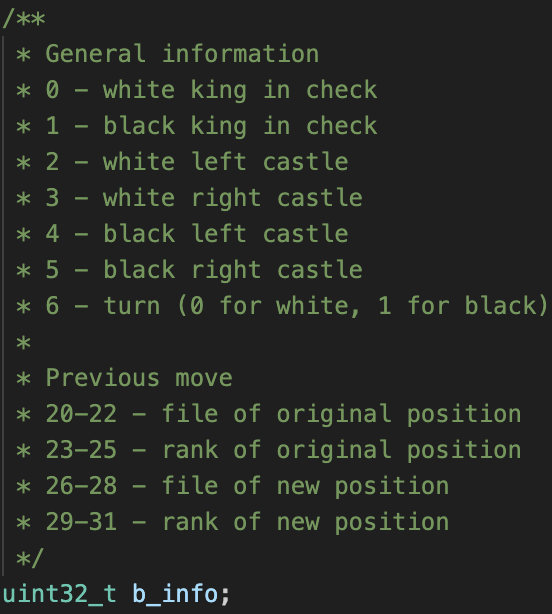
\includegraphics[width=0.8\textwidth]{images/sc1.png}
    % \caption{This is an example image.}
    % \label{fig:example-image}
\end{figure}